\documentclass[12pt]{article}

% Opening
\title{Math 3012 Midterm 2}
\author{Akash Narayanan}
\usepackage{amsmath, amsfonts, amssymb, amsthm, enumitem, tikz}
\usepackage{caption, subcaption, float, marginnote, mathtools, mdframed}

% Solution environment
\newenvironment{solution}{
\begin{mdframed}
  { {\bfseries Solution}: }}{
\end{mdframed}}

\begin{document}

  \maketitle

  \begin{enumerate}
    \item (20 points) Shown below is the diagram of an interval order.
    Use the algorithm taught in class to find an interval representation by computing the down-sets and up-sets in the space provided.
    Then use the First Fit coloring algorithm to find the width \(\omega\) and a partition of the poset into \(\omega\) chains.

    \begin{figure}[H]
      \centering
      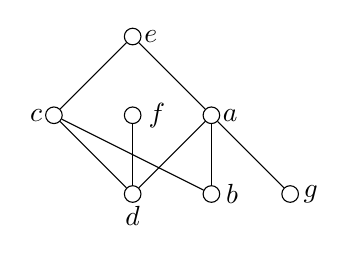
\begin{tikzpicture}
        [scale=1,every node/.style={draw,shape=circle,fill=white,inner sep=0,minimum size=6pt}, every draw/.style={line width=0.25mm, black}]

        \node[label=0:{\(a\)}] (v1) at (0, 0) {};
        \node[label=0:{\(b\)}] (v2) at (0, -1) {};
        \node[label=180:{\(c\)}] (v3) at (-2, 0) {};
        \node[label=270:{\(d\)}] (v4) at (-1, -1) {};
        \node[label=0:{\(e\)}] (v5) at (-1, 1) {};
        \node[label=0:{\(f\)}] (v6) at (-1, 0) {};
        \node[label=0:{\(g\)}] (v7) at (1, -1) {};

        \draw (v1) -- (v2);
        \draw (v1) -- (v4);
        \draw (v1) -- (v5);
        \draw (v1) -- (v7);
        \draw (v2) -- (v3);
        \draw (v3) -- (v4);
        \draw (v3) -- (v5);
        \draw (v4) -- (v6);

      \end{tikzpicture}
    \end{figure}

    \begin{solution}
      \begin{align*}
        D \left( a \right) &= \{b, d, g\} & U \left( a \right) &= \{e\} \\
        D \left( b \right) &= \emptyset & U \left( b \right) &= \{a, c, e\} \\
        D \left( c \right) &= \{b, d\} & U \left( c \right) &= \{e\} \\
        D \left( d \right) &= \emptyset & U \left( d \right) &= \{a, c, e, f\} \\
        D \left( e \right) &= \{a, b, c, d, g\} & U \left( e \right) &= \emptyset \\
        D \left( f \right) &= \{d\} & U \left( f \right) &= \emptyset \\
        D \left( g \right) &= \emptyset & U \left( g \right) &= \{a, e\}
      \end{align*}
      Ranking the down-sets and up-sets, we find the following interval representation:
      \begin{align*}
        I\left( a \right) &= [4, 4] \\
        I\left( b \right) &= [1, 2] \\
        I\left( c \right) &= [3, 4] \\
        I\left( d \right) &= [1, 1] \\
        I\left( e \right) &= [5, 5] \\
        I\left( f \right) &= [2, 5] \\
        I\left( g \right) &= [1, 3]
      \end{align*}
      The corresponding interval graph is shown below, along with a coloring using the First Fit algorithm.

      \begin{figure}[H]
        \centering
        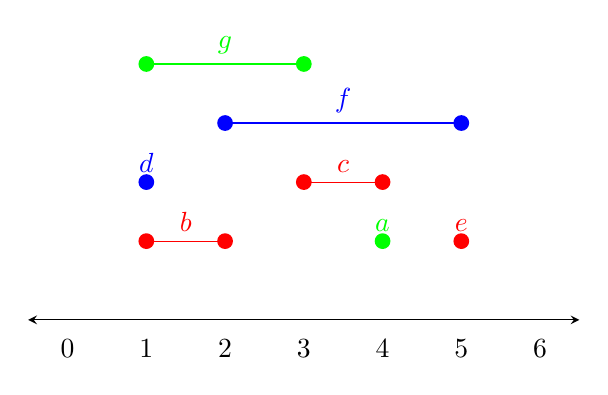
\begin{tikzpicture}

          \draw[green] (4, 0.00) -- node[above] {\(a\)} (4, 0.00);
          \draw[red] (1, 0.00) -- node[above] {\(b\)} (2, 0.00);
          \draw[red] (3, 0.75) -- node[above] {\(c\)} (4, 0.75);
          \draw[blue] (1, 0.75) -- node[above] {\(d\)} (1, 0.75);
          \draw[red] (5, 0.00) -- node[above] {\(e\)} (5, 0.00);
          \draw[blue] (2, 1.50) -- node[above] {\(f\)} (5, 1.50);
          \draw[green] (1, 2.25) -- node[above] {\(g\)} (3, 2.25);

          \fill[green] (4, 0.00) circle (0.1);
          \fill[red] (1, 0.00) circle (0.1); \fill[red] (2, 0.00) circle (0.1);
          \fill[red] (3, 0.75) circle (0.1); \fill[red] (4, 0.75) circle (0.1);
          \fill[blue] (1, 0.75) circle (0.1);
          \fill[red] (5, 0.00) circle (0.1);
          \fill[blue] (2, 1.50) circle (0.1); \fill[blue] (5, 1.50) circle (0.1);
          \fill[green] (1, 2.25) circle (0.1); \fill[green] (3, 2.25) circle (0.1);

          \draw[<->, >=stealth] (-0.5, -1) -- (6.5, -1);

          \node[label=below:{0}] at (0, -1) {};
          \node[label=below:{1}] at (1, -1) {};
          \node[label=below:{2}] at (2, -1) {};
          \node[label=below:{3}] at (3, -1) {};
          \node[label=below:{4}] at (4, -1) {};
          \node[label=below:{5}] at (5, -1) {};
          \node[label=below:{6}] at (6, -1) {};

        \end{tikzpicture}
      \end{figure}

      Since the First Fit algorithm is optimal for interval graphs, the chromatic number is 3.
      In particular, we've partitioned the graph into 3 chains: \(\{a, g\}, \{b, c, e\}, \{d, f\}\).
      Furthermore, there are antichains of size 3, one being \(\{a, c, f\}\).
      Since the width is bounded below by the size of an antichain and bounded above by a partitioning into \(n\) chains, the width of the graph must be 3.
    \end{solution}

    \pagebreak

    \item (20 points) Consider the poset shown below. The ground set is
    \begin{align*}
      X = {a, b, c, d, e, f, g, h}.
    \end{align*}
    Write the reflexive, antisymmetric, and transitive relation on \(X\) which defines this poset.
    \begin{figure}[H]
      \centering
      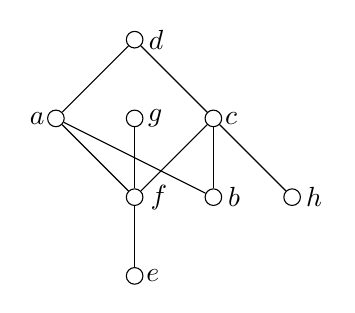
\begin{tikzpicture}
        [scale=1,every node/.style={draw,shape=circle,fill=white,inner sep=0,minimum size=6pt}, every draw/.style={line width=0.25mm, black}]

        \node[label=180:{\(a\)}] (v1) at (0, 0) {};
        \node[label=0:{\(b\)}] (v2) at (2, -1) {};
        \node[label=0:{\(c\)}] (v3) at (2, 0) {};
        \node[label=0:{\(d\)}] (v4) at (1, 1) {};
        \node[label=0:{\(e\)}] (v5) at (1, -2) {};
        \node[label=0:{\(f\)}] (v6) at (1, -1) {};
        \node[label=0:{\(g\)}] (v7) at (1, 0) {};
        \node[label=0:{\(h\)}] (v8) at (3, -1) {};

        \draw (v1) -- (v2);
        \draw (v1) -- (v4);
        \draw (v1) -- (v6);
        \draw (v2) -- (v3);
        \draw (v3) -- (v4);
        \draw (v3) -- (v6);
        \draw (v3) -- (v8);
        \draw (v5) -- (v6);
        \draw (v6) -- (v7);
      \end{tikzpicture}
    \end{figure}

    \begin{solution}
      \begin{align*}
        P = \{ & (a, a), (b, b), (c, c), (d, d), (e, e), (f, f), (g, g), (h, h), \\
               & (a, d), (b, a), (b, c), (b, d), (c, d), (e, a), (e, c), (e, d), \\
               & (e, f), (e, g), (f, a), (f, c), (f, d), (f, g), (h, c), (h, d) \}
      \end{align*}
    \end{solution}

    \pagebreak

    \item (20 points) Let \(2^{15}\) be the poset consisting of all subsets of \(\{1, 2, 3, ..., 15\}\) ordered by inclusion.
    \begin{enumerate}[label=({\alph*})]
      \item (5 points) What is the height of this poset?
      \item (5 points) What is the width of this poset?
      \item (5 points) How many maximal chains does the poset have?
      \item (5 points) How many maximal chains in this poset pass through the set \(\{2, 3, 8, 13\}\)?
    \end{enumerate}

    \begin{solution}
      \begin{enumerate}[label=({\alph*})]
        \item One maximal chain has size 16. Since every maximal chain is maximum, the height is 16.
        \item By Sperner's theorem, the width of the poset is \(C(15, 7) = 6435\).
        \item There are \(15!\) maximal chains formed by adding the elements of the set in any order.
        \item The set \(\{2, 3, 8, 13\}\) has 4 elements. There are \(4! 11!\) maximal chains that pass through the set.
      \end{enumerate}
    \end{solution}

    \pagebreak

    \item (20 points)
    \begin{enumerate}[label=({\alph*})]
      \item (20 points) Let \(X = \{a, b, c, d, e\}\) and let
      \begin{align*}
        P = \{(a, a), (b, b), (c, c), (d, d), (e, e), (d, b), (d, c), (a, e), (a, b), (e, b)\}.
      \end{align*}
      Draw a diagram for the poset \((X, P)\).
      \item (10 points) How many symmetric binary relations are there on \(\{1, 2, ..., n\}\)?
      Of these, how many are reflexive?
    \end{enumerate}

    \begin{solution}
      \begin{enumerate}[label=({\alph*})]
        \item A diagram for the poset \((X, P)\) is shown below.
        \begin{figure}[H]
          \centering
          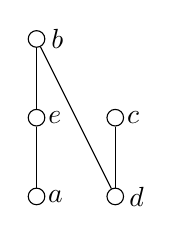
\begin{tikzpicture}
            [scale=1,every node/.style={draw,shape=circle,fill=white,inner sep=0,minimum size=6pt}, every draw/.style={line width=0.25mm, black}]

            \node[label=0:{\(a\)}] (v1) at (0, 0) {};
            \node[label=0:{\(b\)}] (v2) at (0, 2) {};
            \node[label=0:{\(c\)}] (v3) at (1, 1) {};
            \node[label=0:{\(d\)}] (v4) at (1, 0) {};
            \node[label=0:{\(e\)}] (v5) at (0, 1) {};

            \draw (v1) -- (v5);
            \draw (v2) -- (v4);
            \draw (v2) -- (v5);
            \draw (v3) -- (v4);
          \end{tikzpicture}
        \end{figure}

        \item A relation \(R\) is symmetric if whenever \((a, b) \in R\) then \((b, a) \in R\).
        This amounts to choosing 2 element subsets of the base set on \(n\) elements.
        There are precisely \(C(n, 2)\) subsets of size 2. However, this disregards elements of the form \((a, a)\), of which there are \(n\).
        Thus, there are \(C(n, 2) + n = \frac{n(n+1)}{2}\) possible choices for elements of a symmetric relation. A symmetric relation is just a subset of these choices so there are \(2^{\frac{n(n+1)}{2}}\) symmetric relations.

        Of these symmetric relations, a reflexive relation contains \((a, a)\) for all \(a\) in the underlying set.
        That is, we are restricted to choosing distinct pairs of elements to be in our relation.
        Then there are \(2^{C(n, 2)}\) reflexive and symmetric relations.
      \end{enumerate}
    \end{solution}

    \pagebreak

    \item (20 points) Verify Euler's formula for this planar graph.
    \begin{figure}[H]
      \centering
      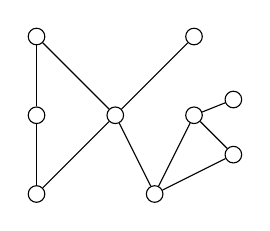
\begin{tikzpicture}
        [scale=1,every node/.style={draw,shape=circle,fill=white,inner sep=0,minimum size=6pt}, every draw/.style={line width=0.25mm, black}]

        \node (v1) at (0, 0) {};
        \node (v2) at (0, 1) {};
        \node (v3) at (0, 2) {};
        \node (v4) at (1, 1) {};
        \node (v5) at (1.5, 0) {};
        \node (v6) at (2, 1) {};
        \node (v7) at (2, 2) {};
        \node (v8) at (2.5, 0.5) {};
        \node (v9) at (2.5, 1.2) {};

        \draw (v1) -- (v2);
        \draw (v1) -- (v4);
        \draw (v2) -- (v3);
        \draw (v3) -- (v4);
        \draw (v4) -- (v5);
        \draw (v4) -- (v7);
        \draw (v5) -- (v6);
        \draw (v5) -- (v8);
        \draw (v6) -- (v8);
        \draw (v6) -- (v9);
      \end{tikzpicture}
    \end{figure}

    \begin{solution}
      Euler's formula is \(V - E + F = 1 + T\) where \(V\) is the number of vertices, \(E\) is the number of edges, \(F\) is the number of faces (including the exterior face), and \(T\) is the number of components.
      This graph is 9 vertices, 10 edges, 3 faces, and 1 component.
      Indeed, \(9 - 10 + 3 = 1 + 1\).
    \end{solution}

  \end{enumerate}
\end{document}
